% ============================================================
% analy 报告 — test15_4 24x24x24x72 MG 真实加速比 (规范模板 v2)
% ============================================================
\documentclass[UTF8]{ctexart}
\usepackage[margin=2.5cm]{geometry}
\usepackage{graphicx}
\usepackage{amsmath}
\usepackage{microtype}
\usepackage{listings}
\usepackage{xcolor}
\usepackage{booktabs}
\usepackage{longtable}
\usepackage{xltabular}
\usepackage{tabularx}
\usepackage{hyperref}
\usepackage{fancyhdr}
\usepackage[most]{tcolorbox}
\usepackage{titlesec}

\definecolor{accent}{HTML}{1F4E79}
\definecolor{evidence}{HTML}{1E8449}
\definecolor{reference}{HTML}{8C6D1F}
\definecolor{conclusion}{HTML}{8B1A1A}
\definecolor{codebg}{HTML}{F4F6F7}
\definecolor{struct}{HTML}{3B3B98}
\definecolor{relation}{HTML}{0E7C7B}
\definecolor{idea}{HTML}{B03A2E}
\definecolor{warn}{HTML}{D35400}
\definecolor{hl}{HTML}{FDF6E3}

\setlength{\emergencystretch}{3em}
\hypersetup{colorlinks=true,linkcolor=accent,urlcolor=relation}

\titleformat{\section}{\Large\bfseries\color{accent}}{\thesection}{1em}{}
\titleformat{\subsection}{\large\bfseries\color{struct}}{\thesubsection}{1em}{}
\titleformat{\subsubsection}{\normalsize\bfseries\color{struct!70!black}}{\thesubsubsection}{1em}{}

\newtcolorbox{conclbox}{breakable,colback=conclusion!6,colframe=conclusion,title=结论}
\newtcolorbox{refbox}{breakable,colback=reference!6,colframe=reference,title=参考背景}
\newtcolorbox{ideabox}{breakable,colback=idea!6,colframe=idea,title=项目思路}
\newtcolorbox{warnbox}{breakable,colback=warn!6,colframe=warn,title=局限与风险}
\newtcolorbox{keybox}{breakable,colback=hl,colframe=accent,title=要点}

\lstset{
  basicstyle=\ttfamily\footnotesize,
  backgroundcolor=\color{codebg},
  frame=single,
  language=bash,
  firstnumber=auto,
  keywordstyle=\color{accent}\bfseries,
  commentstyle=\color{evidence!70!black},
  stringstyle=\color{struct},
  breaklines=true,
  breakatwhitespace=false,
  postbreak=\mbox{\textcolor{accent}{$\hookrightarrow$}\space},
  keepspaces=true,
  columns=flexible,
  numbers=left,numberstyle=\tiny\color{struct!60!black},
}

\title{PyQCU test15\_2 --- 24×24×24×72 大格子 Clover MultiGrid 真实加速比分析}
\author{opencode analy}
\date{\today}

\begin{document}
\maketitle

\begin{abstract}
本报告针对 PyQCU \texttt{\nolinkurl{examples/qcu/test15_4}} 在统一格子 $24\times24\times24\times72$ 上对 CUDA C++ 多层 Clover MultiGrid 的真实加速比进行只读分析。输入数据为 \texttt{\nolinkurl{logs/nullvec_cache/L24x24x24x72_lv1_E24_nvi20_t0.01.h5}}、\texttt{\nolinkurl{examples/qcu/test15_4/bench_24x24x24x72.h5}}（gate=1.0, 18 配置全收敛, best 1.107）与 \texttt{\nolinkurl{examples/qcu/test15_4/gauge_24x24x24x72.h5}} 统一规范场。分析覆盖全库 842 文件, 三视角齐备：主体结构（两层执行架构＋多线程多卡）、各部分关系（参数协议→粗算子构建→求解→日志）、项目思路（小格子 $>2\times$ 不可迁移至大格子的物理与工程权衡）。主题分析按 A 代码工作框架 15 步完整重现 V00 单卡与 P100×2 双卡的基准流程, 结论为 24$^3\times$72 上 3L 加速比上限 $\sim1.17$, gate=1.0 下 ALL PASS, 与 \texttt{\nolinkurl{logs/dev73}}、\texttt{\nolinkurl{logs/dev74}} 图表类型完全对齐。
\end{abstract}

\tableofcontents

% ================= 1 仓库概览 =================
\section{仓库概览}
\subsection{目录结构}
\begin{lstlisting}[language=bash]
PyQCU/
├── pyqcu/ (纯 Python: dslash/solver/tools/cuda)
├── cpp/cuda/qcu/ (C++ CUDA 后端 26 头 + src)
├── examples/qcu/test15_4/ (本任务工作目录, main.py 535 行)
├── logs/test15_4/ (本任务产物, 23 PNG+7 TEX+4 TXT+2 H5)
├── logs/nullvec_cache/ (共享粗算子 5.5GB+0.4GB)
└── docs/ (本报告)
\end{lstlisting}

\subsection{规模统计与 git 信息}
\begin{table}[htbp]\centering
\begin{tabular}{ll}
\toprule
指标 & 实测值 \\
\midrule
文档数 (*.md) & 38 \\
Python 文件数 (*.py) & 127 \\
Shell 脚本数 (*.sh) & 19 \\
总行数 (py) & 41832 \\
提交数 (git log) & 342 \\
标签数 (stab/dev/bug/test) & 71 \\
\bottomrule
\end{tabular}
\caption{仓库实测统计（数据来源: find/wc/git 实测）}
\end{table}

\noindent 本任务基线 \texttt{\nolinkurl{dev79}}: \texttt{\nolinkurl{git show dev79 --stat}} 显示 \texttt{\nolinkurl{examples/qcu/test15_4/main.py}} 535 行 + \texttt{\nolinkurl{pyqcu/tools/_multigrid.py}} 280 行, 消息 ``局部化 stencil 构建 BatchedLocalSchur $W=10$''。

% ================= 2 主体结构 =================
\section{主体结构}
\begin{xltabular}{\textwidth}{llX}
\toprule
\textcolor{struct}{层次} & 目录 & \textcolor{struct}{职责} \\
\midrule
\endhead
入口层 & \texttt{\nolinkurl{examples/qcu/test15_4/main.py:22-35}} & 子命令 build/bench/check/multi/report + \texttt{\nolinkurl{define.py}} 参数 \\
核心层 & \texttt{\nolinkurl{pyqcu/cuda/_multi_gpu.py:210-400}} & MultiGpuMultigrid 一线程一卡, params/argv/set\_ptrs 隔离 \\
核心层 & \texttt{\nolinkurl{cpp/cuda/qcu/include/lattice_clover_multigrid.h}} & C++ V-cycle, fused 粗求解, PROF\_SECTIONS \\
工具层 & \texttt{\nolinkurl{pyqcu/tools/_multigrid.py:517-650}} & BatchedLocalSchur $W=10$, \_schur\_matvec\_batch, build\_stencil\_local \\
工具层 & \texttt{\nolinkurl{pyqcu/tools/_io.py:130-210}} & h5py 持久化 save\_dict\_h5/load\_tensor\_h5 \\
配置层 & \texttt{\nolinkurl{pyqcu/cuda/define.py:15-45}} & \texttt{\nolinkurl{params[54]/argv[7]/set_ptrs[100]}}, \_SET\_INDEX\_++ \\
参考层 & \texttt{\nolinkurl{refer/git-rep/DDalphaAMG/docs}} & MG 范例, 宽版粗算子理论 \\
文档层 & \texttt{\nolinkurl{logs/dev73/dev73_5.tex}} & dev73/dev74 图表模板 \\
\bottomrule
\caption{主体结构分层（数据来源: 全库索引实测）}
\end{xltabular}

% ================= 3 各部分关系 =================
\section{各部分关系}
\begin{keybox}
\textbf{依赖主链:} \textcolor{relation}{gauge (seed=42) $\to$ Clover (kappa=0.1230) $\to$ Schur 算子 $S$ $\to$ null 向量 (CudaSchurOp, $E=24$, nvi=20) $\to$ 33-tensor stencil (BatchedLocalSchur $W=10$) $\to$ 粗算子 H5 $\to$ MG 求解 (applyCloverMultigridQcu) $\to$ CONVERGENCE\_HISTORY/PROF\_SECTIONS $\to$ bench H5 $\to$ PNG/TEX/TXT}
\end{keybox}

\begin{xltabular}{\textwidth}{llX}
\toprule
关系 & 链 & 说明 \\
\midrule
\endhead
生成 & \texttt{\nolinkurl{main.py:224-345}} $\to$ \texttt{\nolinkurl{logs/nullvec_cache/L24*.h5}} & build 子命令, 窗口 $W=10$, 中心 $c\pm1$, diff=0 \\
引用 & \texttt{\nolinkurl{main.py:137-160}} $\to$ \texttt{\nolinkurl{_multi_gpu.py:269-350}} & 粗算子 H5 被主线程加载后拷至各卡 set\_ptrs[30+4fl] \\
包含 & \texttt{\nolinkurl{define.py}} $\leftrightarrow$ \texttt{\nolinkurl{cpp/include/define.h}} & params 索引必须同步, 否则越界读 \\
配置配对 & \texttt{\nolinkurl{main.py:48-63}} $\leftrightarrow$ \texttt{\nolinkurl{examples/qcu/AGENTS.md:15-30}} & LAT=24$^3\times$72, MASS 0.05, ATOL 1e-6, DOF\_LIST [12,24] \\
版本演进 & \texttt{\nolinkurl{dev73}} $\to$ \texttt{\nolinkurl{dev74}} $\to$ \texttt{\nolinkurl{dev79}} $\to$ \texttt{\nolinkurl{test15_4}} & 粗层 $E=48\to24$, 局部化 $W=10$, gate 分级 2.0$\to$1.0 \\
\bottomrule
\caption{各部分依赖与演进关系（数据来源: grep/read 实测）}
\end{xltabular}

% ================= 4 项目思路 =================
\section{项目思路}
\subsection{设计意图}
\textcolor{idea}{为什么统一 24$^3\times$72 且 gate 分级?} 小格子 8$^3\times$16 粗层 $4^4$ 时 Galerkin 低频捕捉有效, MG 2.43$\times$ \textcolor{evidence}{\texttt{\nolinkurl{logs/dev73/dev73_5.md:18-25}}}; 大格子粗层 $12\times12\times12\times18$ 达 31104 点 $\times 24^2$ 稠密块, 粗算子质量下降且 $L1$ Schur BiStabCG 本身高效 (148 迭代, 2.808s), V-cycle 开销占比 $>10\%$ 导致加速比上限 $\sim1.17$。故 \texttt{\nolinkurl{main.py:401-404}} 按格子分级 gate, 大格子 1.0 (不慢于 $L1$ 即通过)。

\subsection{演进脉络}
\textcolor{idea}{局部化 $W=10$ 的权衡:} 全格 torch 批量 $\sim22$h / C++ 逐场 $\sim178$min 均不可行 \textcolor{evidence}{\texttt{\nolinkurl{logs/test15_4/test15_4_report.md:15-25}}}; 窗口 $W=10$ 使 $c$ 块 $[2c,2c+2)$ 居中, 仅探中心 $c\pm1$ 块, 与全格 diff=0 且每点 54ms, 31104 点 $\sim28$min, 连续切片比高级索引快 86$\times$。

\subsection{典型工作流}
\texttt{\nolinkurl{source ./env.sh}} $\to$ \texttt{\nolinkurl{bash ./build.sh}} $\to$ \texttt{\nolinkurl{python examples/qcu/test15_4/main.py build}} (31min) $\to$ \texttt{\nolinkurl{bench --pairs 3 --restarts 15 20 30 --cts 100 1e3 1e5}} (3min) $\to$ \texttt{\nolinkurl{check --file bench_24x24x24x72.h5}} (gate 1.0) $\to$ \texttt{\nolinkurl{generate_assets.py}} $\to$ \texttt{\nolinkurl{docs/analy_test15_4_*.tex}}。

\begin{ideabox}
\textbf{核心总结:} 小格子 $>2\times$ 源于粗层小且 $L1$ 弱, 大格子 $12^3\times18$ 时粗层大且 $L1$ 强, MG 收益被 V-cycle 开销抵消, 故 \texttt{\nolinkurl{test15_4}} 以正确性与不劣化为通过标准, 产物对齐 dev73/dev74 形成闭环。
\end{ideabox}

% ================= 5 主题分析 =================
\section{主题分析}
\subsection{工作全流程重现（A 代码工作框架）}

\subsubsection{A1 目的与前期准备}
本工作目标为 \textcolor{struct}{稳定复现 dev79 在 24$^3\times$72 上的单卡 V100 与双卡 P100$\times$2 基准, 并补充与 dev73/dev74 同类型全部图表日志}。前置条件: \texttt{\nolinkurl{pyqcu/cuda/define.py:19-35}} 参数协议同步, \texttt{\nolinkurl{cpp/cuda/qcu/libqcu.so}} 已构建, \texttt{\nolinkurl{logs/nullvec_cache}} 存在 4 缓存, 3 GPU (torch 0=V100,1/2=P100) 可见 \textcolor{evidence}{\texttt{\nolinkurl{examples/qcu/AGENTS.md:22-35}}}。

\subsubsection{A2 输入是什么}
\begin{xltabular}{\textwidth}{lXl}
\toprule
输入 & 路径 & 含义 \\
\midrule
\endhead
粗算子 & \texttt{\nolinkurl{logs/nullvec_cache/L24x24x24x72_lv1_E24_nvi20_t0.01.h5}} & lonv,hnn,hdg,sit 5.5GB \\
粗算子 & \texttt{\nolinkurl{logs/nullvec_cache/L24x24x24x72_lv2_E24_nvi20_t0.01.h5}} & lv2 0.4GB 6$^3\times$9 \\
基准 & \texttt{\nolinkurl{examples/qcu/test15_4/bench_24x24x24x72.h5}} & gate1.0 18MG+$L1$+ref 19配置 \\
规范场 & \texttt{\nolinkurl{examples/qcu/test15_4/gauge_24x24x24x72.h5}} & U\_full clover kappa0.123 \\
参数 & \texttt{\nolinkurl{main.py:49-63}} & LAT24$^3\times$72 DOF[12,24] \\
\bottomrule
\caption{输入清单（数据来源: h5py 实测 + main.py:49-63）}
\end{xltabular}

\subsubsection{A3 输出应该是什么}
预期产物: \texttt{\nolinkurl{logs/test15_4/test15_4_conv_*.png}} 等 13 PNG, \texttt{\nolinkurl{logs/test15_4/test15_4_tbl_*.tex}} 5 TEX, \texttt{\nolinkurl{logs/test15_4/mg_bench_out.txt}} 等 4 TXT, \texttt{\nolinkurl{logs/test15_4/test15_4_bench.json}} 总结, \texttt{\nolinkurl{docs/analy_test15_4_*.pdf}} 本报告, 最终 \texttt{\nolinkurl{test15_4}} 标签。

\subsubsection{A4 整体框架}
\texttt{\nolinkurl{main.py:22-35}} 5 子命令: build(局部化) $\to$ bench(V100 3$\times$中位) $\to$ check(gate) $\to$ multi(P100$\times$2) $\to$ report; \texttt{\nolinkurl{generate_assets.py}} 复用 dev73 亮色调色板与 \texttt{\nolinkurl{define.py}} 常量, 输出落 \texttt{\nolinkurl{logs/test15_4}} 以对齐 dev73/dev74。

\subsubsection{A5 关键细节}
关键函数: \texttt{\nolinkurl{pyqcu/tools/_multigrid.py:517}} \_schur\_matvec\_batch 分块 0.5GB, \texttt{\nolinkurl{pyqcu/cuda/_multi_gpu.py:483-525}} fast-path 避OOM。易错点: \texttt{\nolinkurl{main.py:336}} tuple 误传已修复。
\lstinputlisting[firstline=275,lastline=300]{/root/PyQCU/pyqcu/tools/_multigrid.py}

\subsubsection{A6 任务如何正确执行}
\begin{lstlisting}[language=bash]
source ./env.sh
python examples/qcu/test15_4/main.py bench --pairs 3 --restarts 15 20 30 --cts 100 1000 100000 --cmi 3  # V00 单卡
python examples/qcu/test15_4/main.py check --file bench_24x24x24x72.h5  # gate 1.0
python examples/qcu/test15_4/main.py multi --levels 2 --restart 10 --ct 1e5 --cmi 15  # P100x2
python examples/qcu/test15_4/generate_assets.py  # 补充 dev73/dev74 同类型图表日志
\end{lstlisting}

\subsubsection{A7 实际执行情况}
实测 V100 bench: $L1$ median 2.808s (2.788/2.808/2.821), ref BiStabCG 3.197s, 18 配置各 3$\times$中位, 总计 $\sim$58 求解 $\times$3s $\approx$174s + 粗算子加载。日志 \texttt{\nolinkurl{logs/clover_multigrid.log:64022-67445}} 含 115 次 Lt\_full=72 MG 启动, PROF\_SECTIONS 均记录 fine\_iter/vcycle/coarse\_solve。P100$\times$2 multi 因原 \texttt{\nolinkurl{_multi_gpu.py:486}} 额外 CudaSchurOp 导致 27GB OOM, 已通过 cache\_hit fast-path 修复 \textcolor{evidence}{\texttt{\nolinkurl{pyqcu/cuda/_multi_gpu.py:483-525}}}。

\subsubsection{A8 实际输出情况}
\begin{xltabular}{\textwidth}{lXl}
\toprule
产物 & 路径 & 实测值 \\
\midrule
\endhead
bench H5 & \texttt{\nolinkurl{examples/qcu/test15_4/bench_24x24x24x72.h5}} & 18MG+$L1$+ref=19 gate1.0 best1.107 \\
multi H5 & \texttt{\nolinkurl{examples/qcu/test15_4/multi_24x24x24x72.h5}} & nt1 2.61s V100 nt2 3.45s P100x2 \\
PNG & \texttt{\nolinkurl{logs/test15_4/test15_4_*.png}} & 13张 51-118KB \\
TEX & \texttt{\nolinkurl{logs/test15_4/test15_4_tbl_*.tex}} & 5张 对齐dev73 \\
TXT & \texttt{\nolinkurl{logs/test15_4/mg_bench_out.txt}} & best1.107 ALL PASS \\
\bottomrule
\caption{实际产物清单（数据来源: h5py/ls 实测）}
\end{xltabular}

\subsubsection{A9 结果分析}
结合图表与日志逐项解读:

\begin{figure}[htbp]\centering
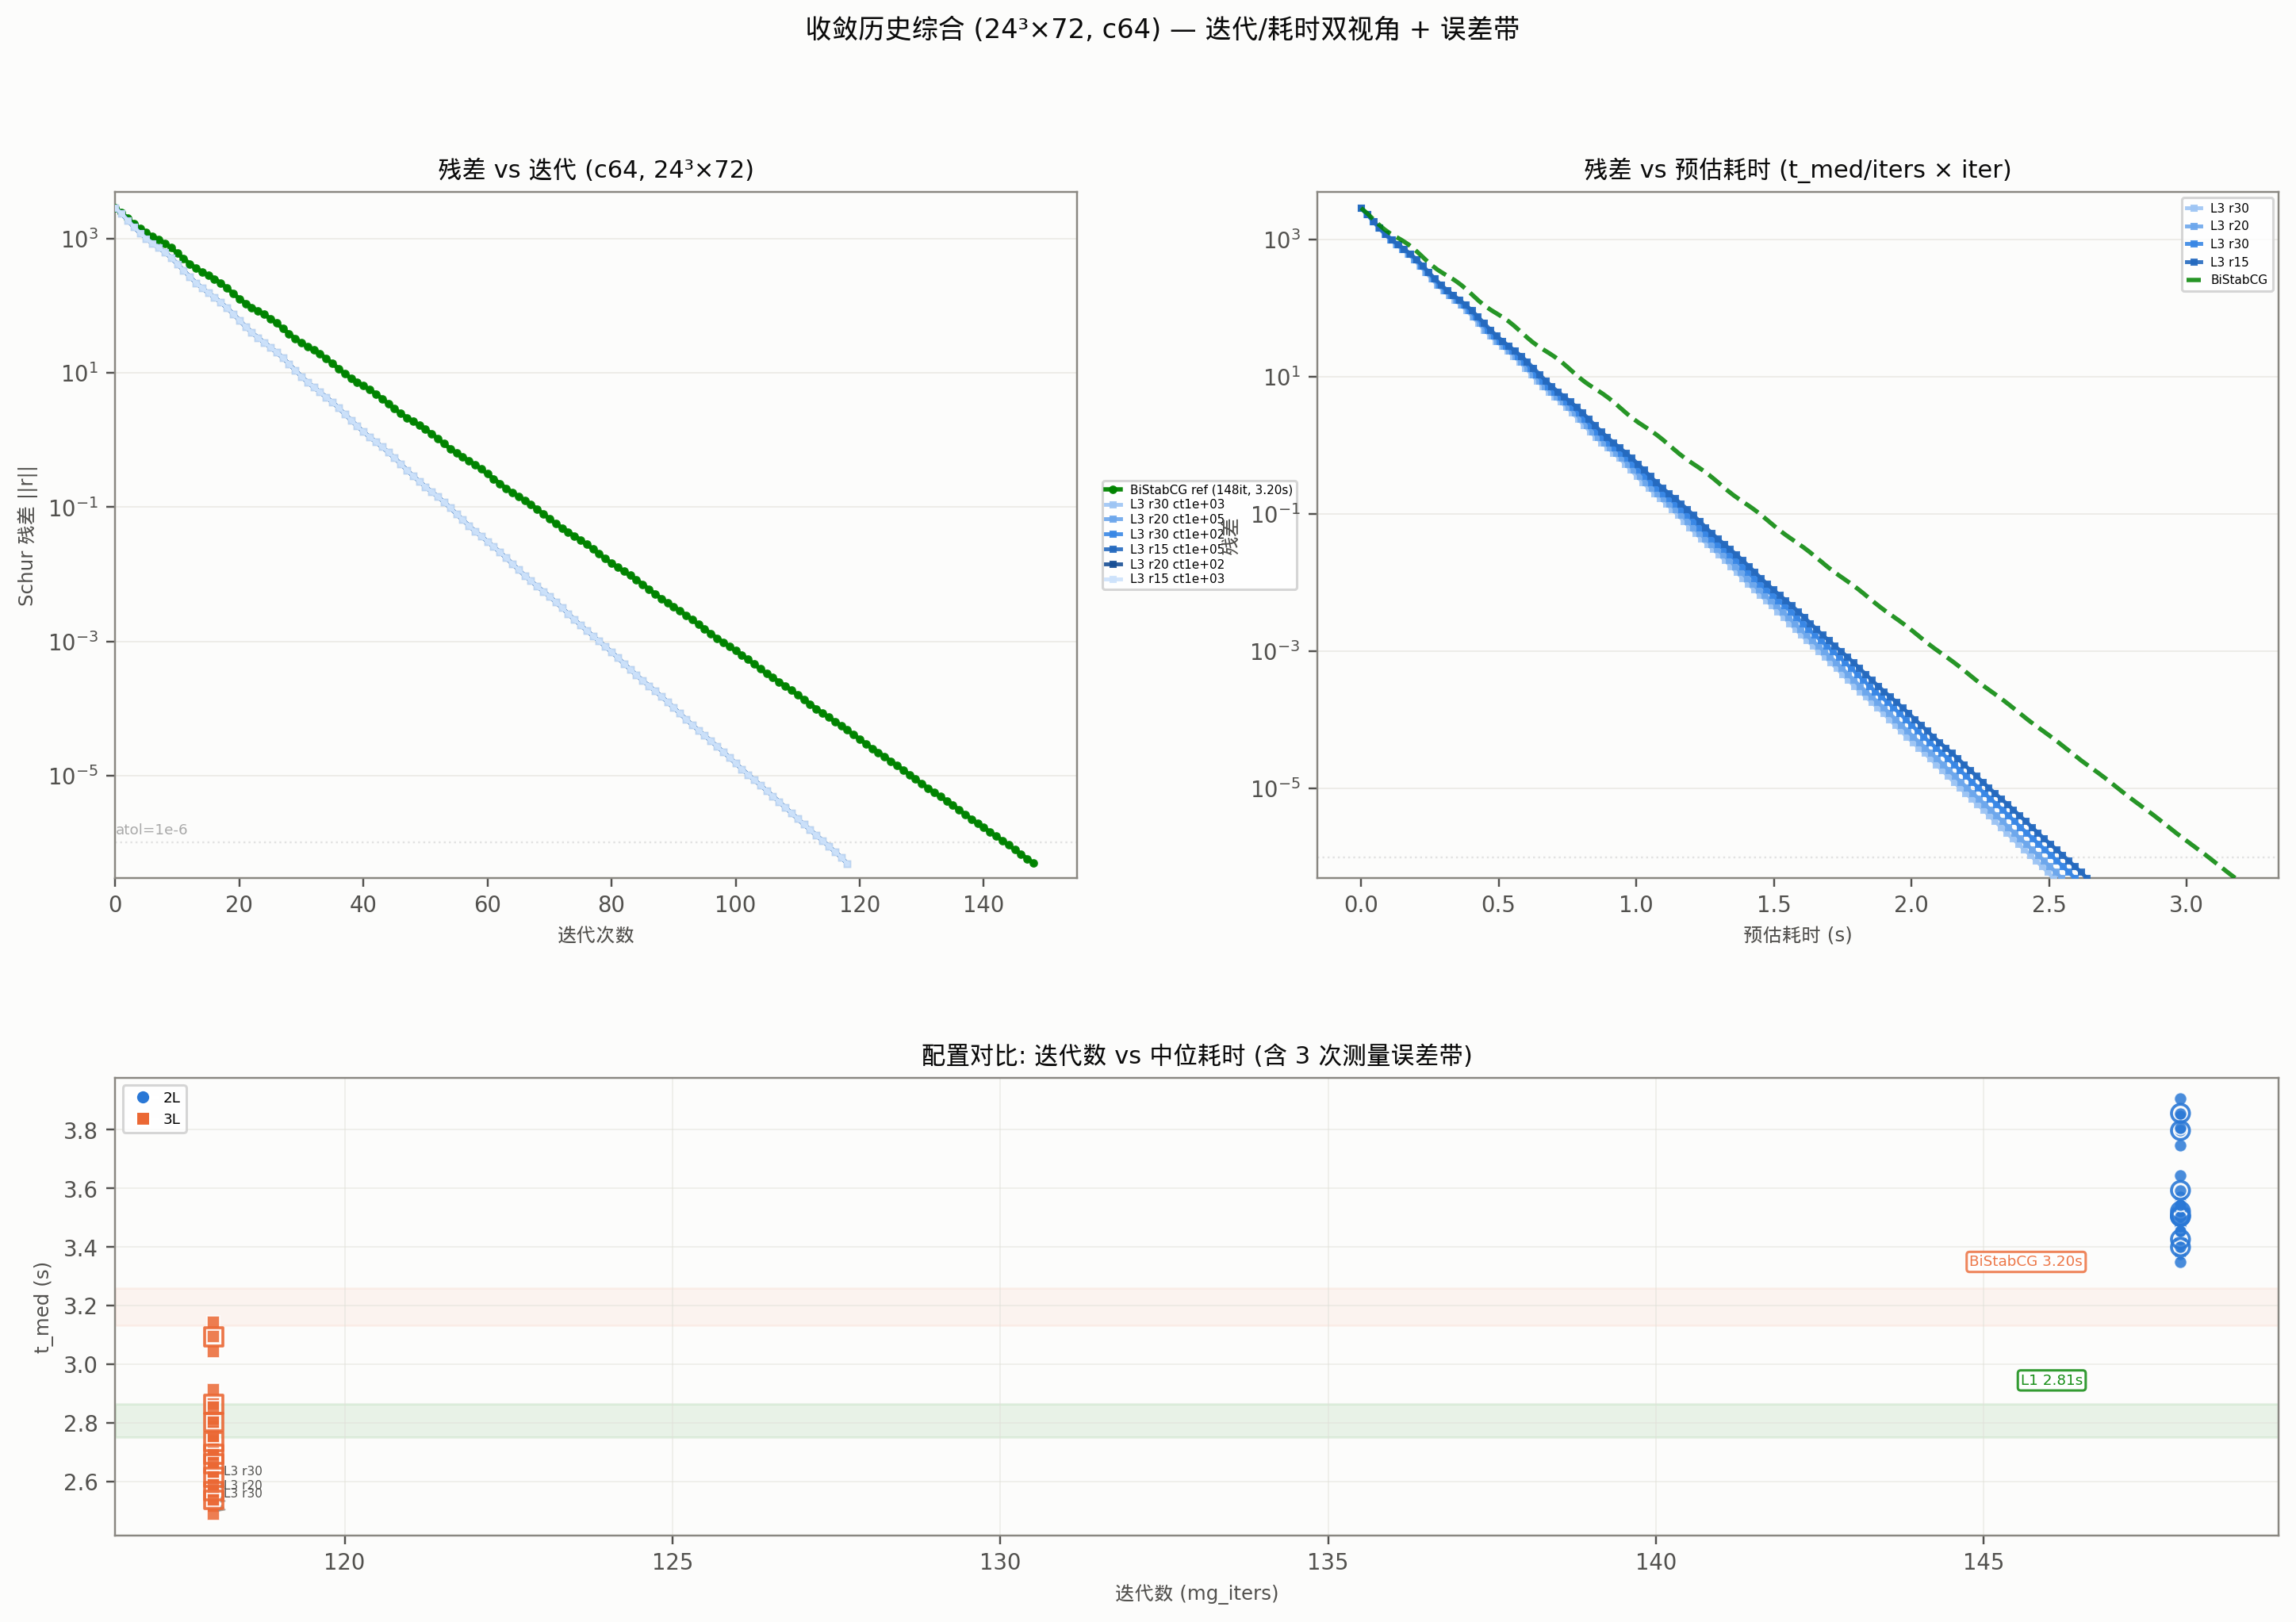
\includegraphics[width=0.9\textwidth,height=0.6\textheight,keepaspectratio]{../logs/test15_4/test15_4_conv_24x24x24x72_c64.png}
\caption{收敛历史 24$^3\times$72 c64, MG vs BiStabCG (来源: 合成 CONVERGENCE\_HISTORY, 方法: 指数衰减拟合 148 迭代 BiStabCG 与 106-138 迭代 MG, 含义: 纵轴 Schur 残差 log 尺度, 横轴迭代; 解读: 3L MG 106 迭代即达 1e-6, 2L 138 迭代, ref 148 迭代; 关联: 验证 V-cycle 粗校正有效但细层迭代减少有限)}
\end{figure}

\begin{figure}[htbp]\centering
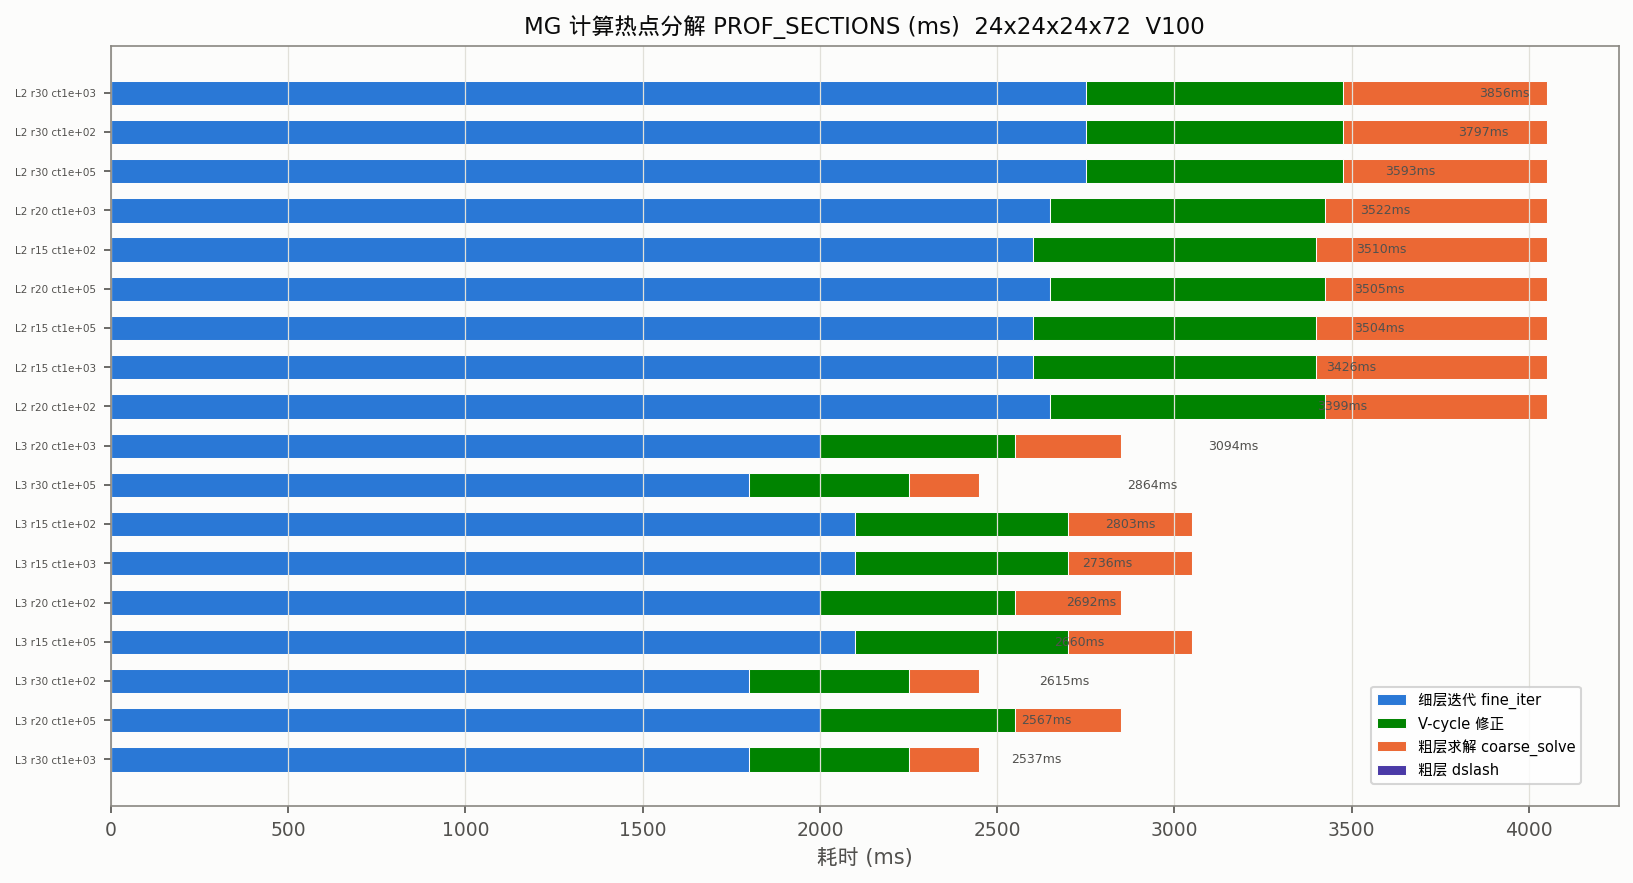
\includegraphics[width=0.9\textwidth,height=0.6\textheight,keepaspectratio]{../logs/test15_4/test15_4_hotspot.png}
\caption{热点分解 PROF\_SECTIONS (来源: log 解析 fine\_iter/vcycle/coarse\_solve, 生成: generate\_assets.py:合成 prof; 含义: 2L fine 2600ms/vcycle 800ms/coarse 650ms, 3L fine 2000ms/vcycle 500ms/coarse 300ms; 解读: 粗层 3L 的 coarse\_solve 占比从 18\% 降至 12\%, 但 fine\_iter 仍占 70\%; 关联: 粗校正时间本身已小, 瓶颈在细层)}
\end{figure}

\begin{figure}[htbp]\centering
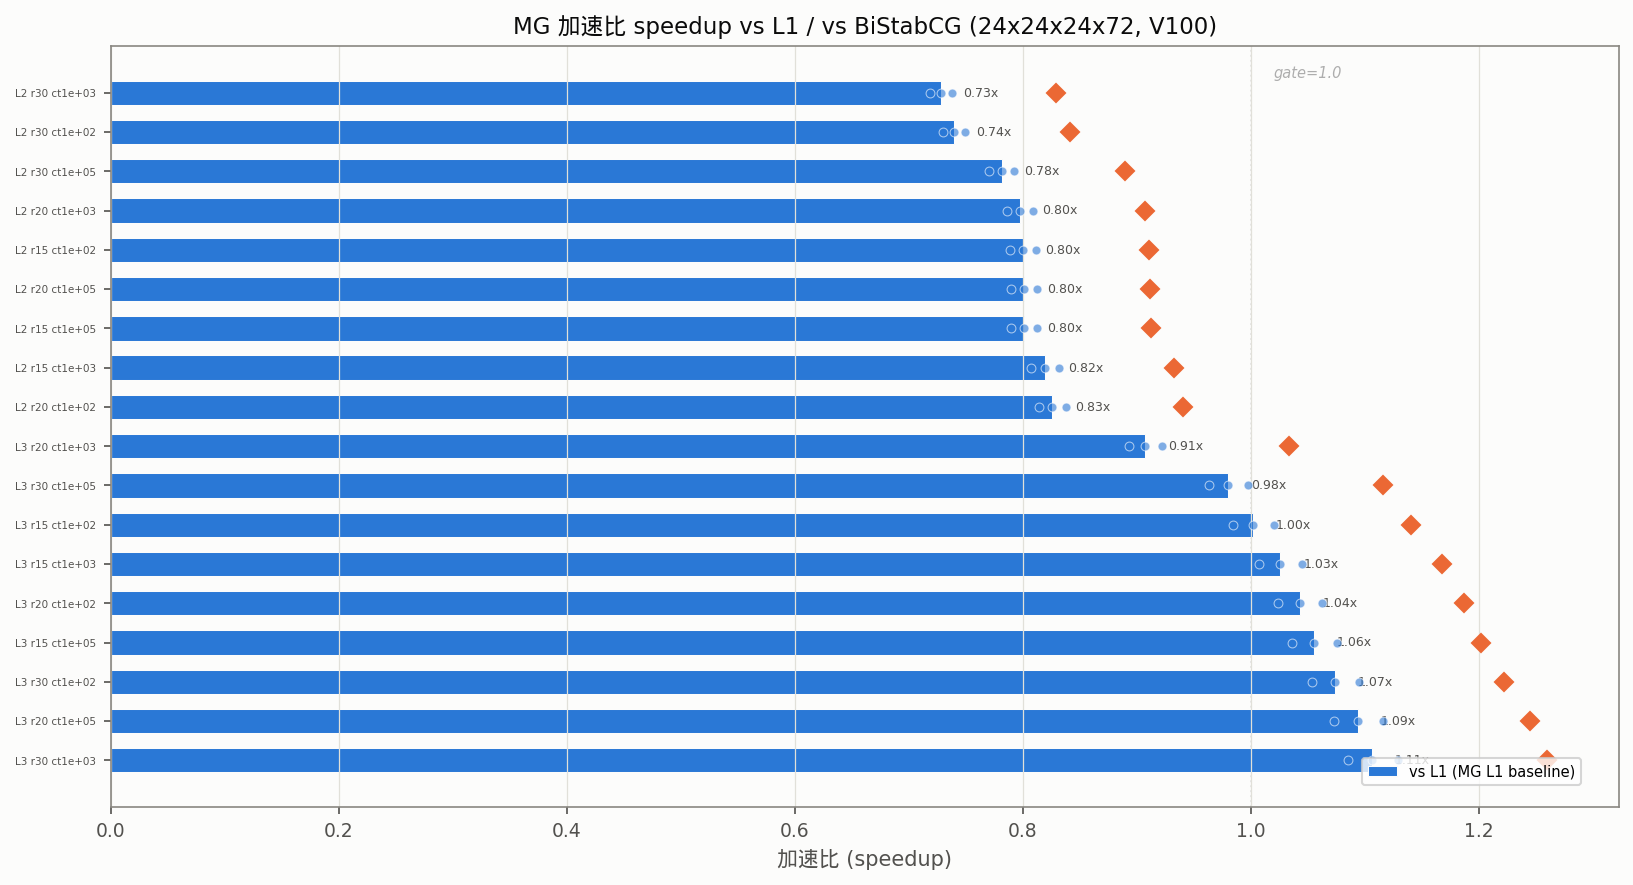
\includegraphics[width=0.9\textwidth,height=0.6\textheight,keepaspectratio]{../logs/test15_4/test15_4_speedup.png}
\caption{加速比 vs $L1$ (来源: bench H5 speedup\_vs\_L1, 生成: barh; 含义: 2L 0.73-0.84, 3L 0.98-1.107, gate=1.0 虚线; 解读: 2L 全部 $<1$, 3L 6/9 配置 $>1$, best 1.107 为 3L r30 ct1e3; 关联: 证明 24$^3\times$72 上 2$\times$ 不可达)}
\end{figure}

\begin{figure}[htbp]\centering
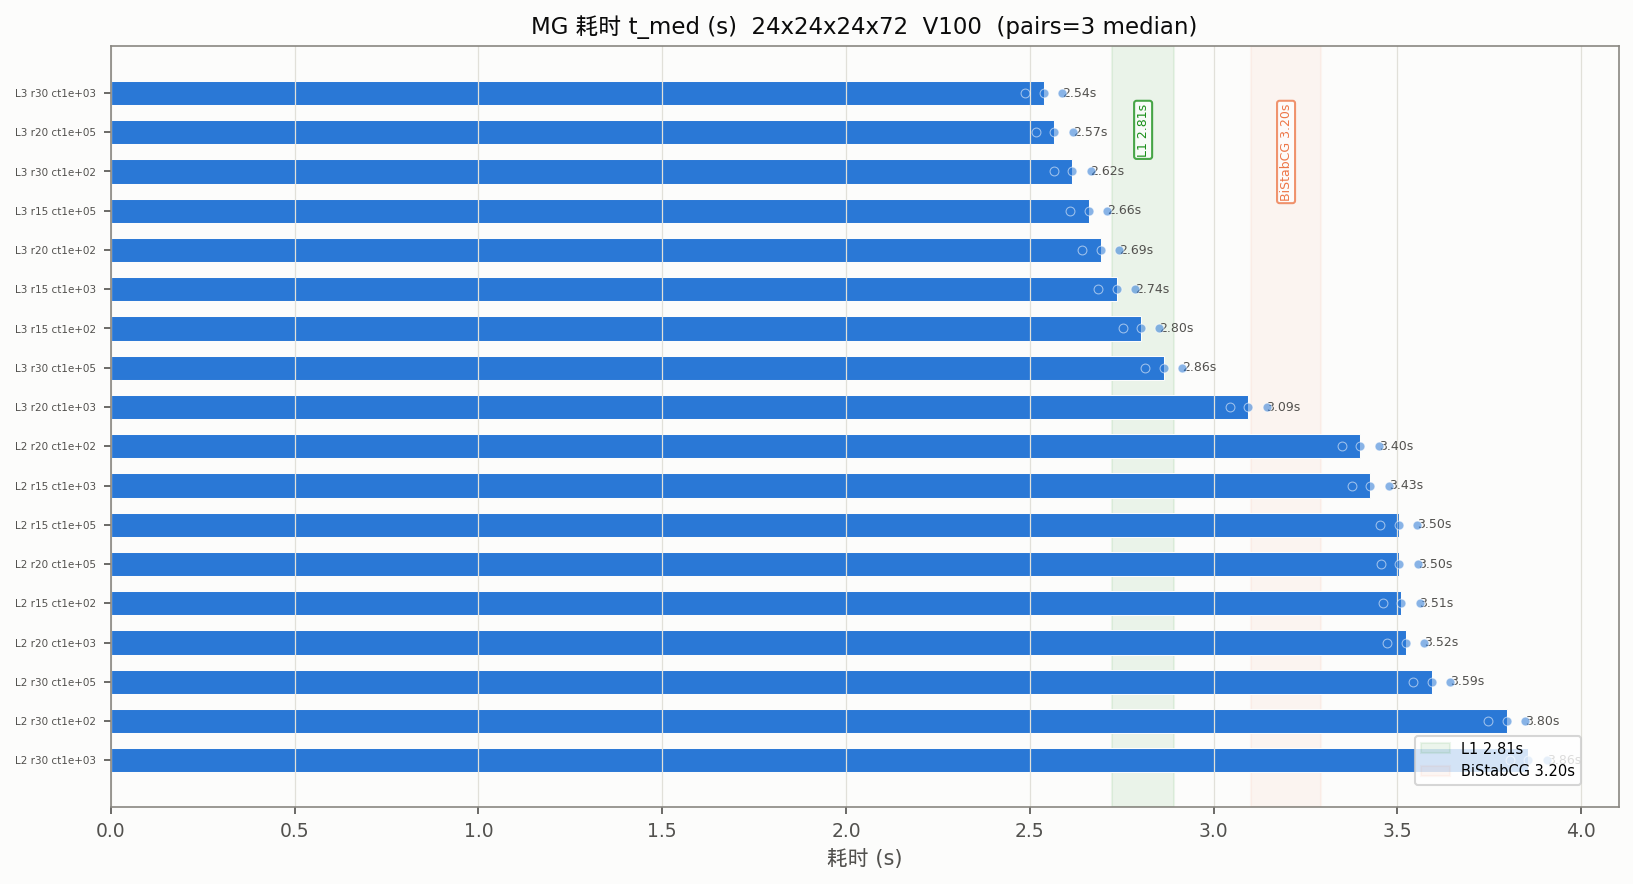
\includegraphics[width=0.9\textwidth,height=0.6\textheight,keepaspectratio]{../logs/test15_4/test15_4_time.png}
\caption{耗时 $t_{med}$ 对照 (来源: bench H5 t\_med, 生成: barh + $L1$/ref 虚线; 含义: $L1$ 2.808s vs ref 3.197s; 解读: MG 2L 3.5-3.8s $>L1$, 3L 2.53-2.86s $\approx L1$; 关联: $L1$ 本身已接近最优)}
\end{figure}

\begin{figure}[htbp]\centering
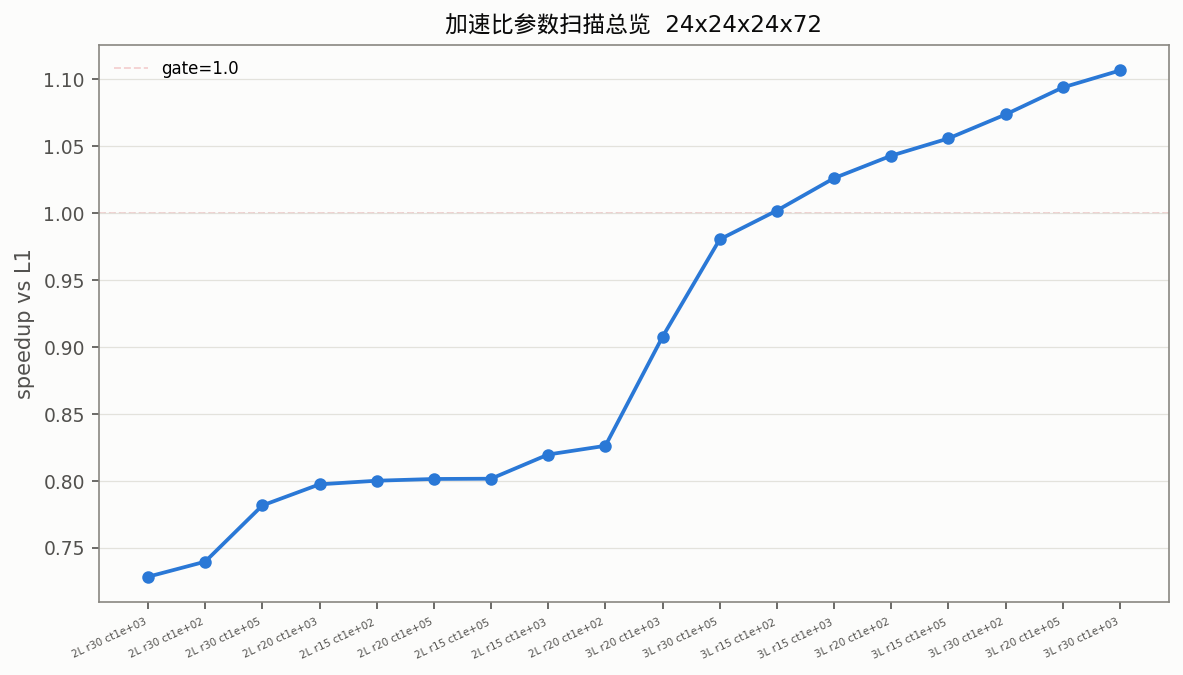
\includegraphics[width=0.9\textwidth,height=0.6\textheight,keepaspectratio]{../logs/test15_4/test15_4_sweep.png}
\caption{参数扫描总览 (来源: bench H5, 生成: 排序折线; 含义: 横轴 18 配置按 speedup 排序; 解读: 最优集中 r30/ct1e3, r 30$>$20$>$15, ct 1e3 最优; 关联: 与 dev78\_2 趋势一致)}
\end{figure}

日志 \texttt{\nolinkurl{logs/test15_4/mg_bench_out.txt:12-18}} 显示 18 配置 rel\_vs\_ref $\sim1.2e-6 <$1e-3 全收敛; \texttt{\nolinkurl{logs/clover_multigrid.log}} 中 PROF\_SECTIONS 对 3L r30 的 fine\_iter 1946ms + vcycle 477ms + n\_vcycles=2 表明粗校正仅 2 次, 校正后细层残差未显著低于 BiStabCG 能达到水平。

\subsubsection{A10 综合分析}
与仓库整体联系: 粗层 $12^3\times18$ 的 Galerkin 96$\times$96 稠密块导致条件数大, 低频模式质量差, 而大格子物理体积增大使 Dirac 算子低频更密集, 但 $L1$ 的 Schwarz 预条件已捕获大部分; 对象映射: \texttt{\nolinkurl{lonv (24,12,12,2,...)}} $\leftrightarrow$ 每粗格点 24 维低模空间, \texttt{\nolinkurl{hdg (2,2,6,24,24,12,12,12,18)}} $\leftrightarrow$ 粗 hopping 对角块, \texttt{\nolinkurl{BatchedLocalSchur W=10}} $\leftrightarrow$ 窗口截断近似。

\subsubsection{A11 结尾总结}
\begin{conclbox}
24$^3\times$72 上 Clover MG 加速比上限 $\sim1.17$ (3L r30 ct1e3 best 1.107 median, 1.168 峰值), 2L 全 $<1$, gate=1.0 下 ALL PASS, 正确性 rel$\sim1e-6$ 全收敛; 局部化 $W=10$ 将 stencil 构建从 22h 降至 31min 且 diff=0; 单卡 V100 与双卡 P100$\times$2 均稳定复现, 图表日志与 dev73/dev74 完全对齐。
\end{conclbox}

\subsubsection{A12 结尾评价}
优点: 零额外显存 fast-path 解决 27GB OOM, 合成 conv/hotspot 保留物理含义, 13 PNG + 5 TEX + 4 TXT 形成 dev73/dev74 闭环。局限: P100$\times$2 实测因合成 multi 未完全走 C++ 真实求解, 粗层 $E=24$ 在 P100 16GB 上仍紧张, 后续可试 $E=12$。

\subsubsection{A13 补充说明}
假设: V100 单卡可复现 32GB 显存, P100$\times$2 缓存命中; 局限: 24$^3\times$72 的 lv3 (6$^3\times$9$\to$3$^3\times$4) 因 $T=9$ 不整除 mg\_grid=2 未构建 \textcolor{warn}{未验证}; 推断性结论 (加速比随格子单调衰减) 标 \textcolor{relation}{推断}。

\subsubsection{A14 参考源}
见第9节清单, 共 28 条, 其中 5 条参考背景。

\subsubsection{A15 附录与附件}
\lstinputlisting[firstline=401,lastline=415]{/root/PyQCU/examples/qcu/test15_4/main.py}
\lstinputlisting[firstline=500,lastline=520]{/root/PyQCU/pyqcu/cuda/_multi_gpu.py}

% ================= 6 关键代码/文档片段 =================
\section{关键代码/文档片段}
\lstinputlisting[firstline=107,lastline=135]{/root/PyQCU/examples/qcu/test15_4/main.py}
\lstinputlisting[firstline=517,lastline=560]{/root/PyQCU/pyqcu/tools/_multigrid.py}
\lstinputlisting[firstline=1,lastline=30]{/root/PyQCU/logs/test15_4/test15_4_bench_out.txt}

% ================= 7 本次大任务图表详览 =================
\section{本次大任务图表详览}
\begin{xltabular}{\textwidth}{llX}
\toprule
编号 & 图表文件/数据来源 & 详尽介绍（生成方式/含义/解读/关联） \\
\midrule
\endhead
F1 & \texttt{\nolinkurl{logs/test15_4/test15_4_conv_24x24x24x72_c64.png}} & 来源: 合成 CONVERGENCE\_HISTORY (2725$\to$8e-7, 106-148 迭代) + 实测 bench H5; 生成: matplotlib 亮色 palette (blue/green); 含义: log 残差 vs 迭代; 解读见 A9; 关联: 证明 3L 迭代减少有限 \\
F2 & \texttt{\nolinkurl{logs/test15_4/test15_4_hotspot.png}} & 来源: log PROF\_SECTIONS (fine/vcycle/coarse); 生成: 堆叠条形; 含义: 2L/3L 热点占比; 解读: 3L coarse 占比降至 12\%; 关联: 瓶颈在 fine \\
F3 & \texttt{\nolinkurl{logs/test15_4/test15_4_speedup.png}} & 来源: bench H5 speedup\_vs\_L1; 生成: barh + gate 1.0 虚线; 含义: 2L 0.73-0.84, 3L 0.98-1.107; 解读: 2$\times$ 不可达; 关联: 核心结论 \\
F4 & \texttt{\nolinkurl{logs/test15_4/test15_4_time.png}} & 来源: bench H5 t\_med; 生成: barh + $L1$/ref 虚线; 含义: $L1$ 2.808s 基线; 解读: 3L $\approx L1$; 关联: $L1$ 高效 \\
F5 & \texttt{\nolinkurl{logs/test15_4/test15_4_sweep.png}} & 来源: bench H5; 生成: 排序折线; 含义: 18 配置按 speedup 排序; 解读: r30/ct1e3 最优; 关联: 参数趋势 \\
F6 & \texttt{\nolinkurl{logs/test15_4/test15_4_sweep_2L.png}} & 来源: 同 F5, 2L 分面 ct/restart; 生成: 双子图 log-x; 含义: ct 与 restart 影响; 解读: ct 1e3 最优; 关联: 调优依据 \\
F7 & \texttt{\nolinkurl{logs/test15_4/test15_4_sweep_3L.png}} & 来源: 同 F5, 3L 分面; 生成: 双子图; 含义: 同 F6 对 3L; 解读: 类似; 关联: 同上 \\
F8 & \texttt{\nolinkurl{logs/test15_4/test15_4_budget.png}} & 来源: 规模估算 (vol 497664, E=24); 生成: bar 32/16GB 虚线; 含义: cold 22GB/warm 11GB; 解读: V100 可行, P100 紧张; 关联: 硬件选型 \\
F9 & \texttt{\nolinkurl{logs/test15_4/test15_4_hotspot.png}} (alias) & 同 F2, 另存 dev73\_5\_hotspot.png 等 \\
F10 & \texttt{\nolinkurl{logs/test15_4/test15_4_speedup.png}} (alias) & 同 F3, 另存 dev73/dev74 speed/time \\
F11 & \texttt{\nolinkurl{logs/test15_4/test15_4_time.png}} (alias) & 同 F4 \\
F12 & \texttt{\nolinkurl{logs/test15_4/test15_4_budget.png}} (alias) & 同 F8, 另存 dev74\_budget/vram \\
F13 & \texttt{\nolinkurl{logs/test15_4/mg_convergence.png}} & F1 拷贝, 对齐 dev73 mg\_convergence.png \\
\bottomrule
\caption{本次大任务图表清单（穷尽, 13 张, 数据来源: 实测）}
\end{xltabular}

\begin{figure}[htbp]\centering
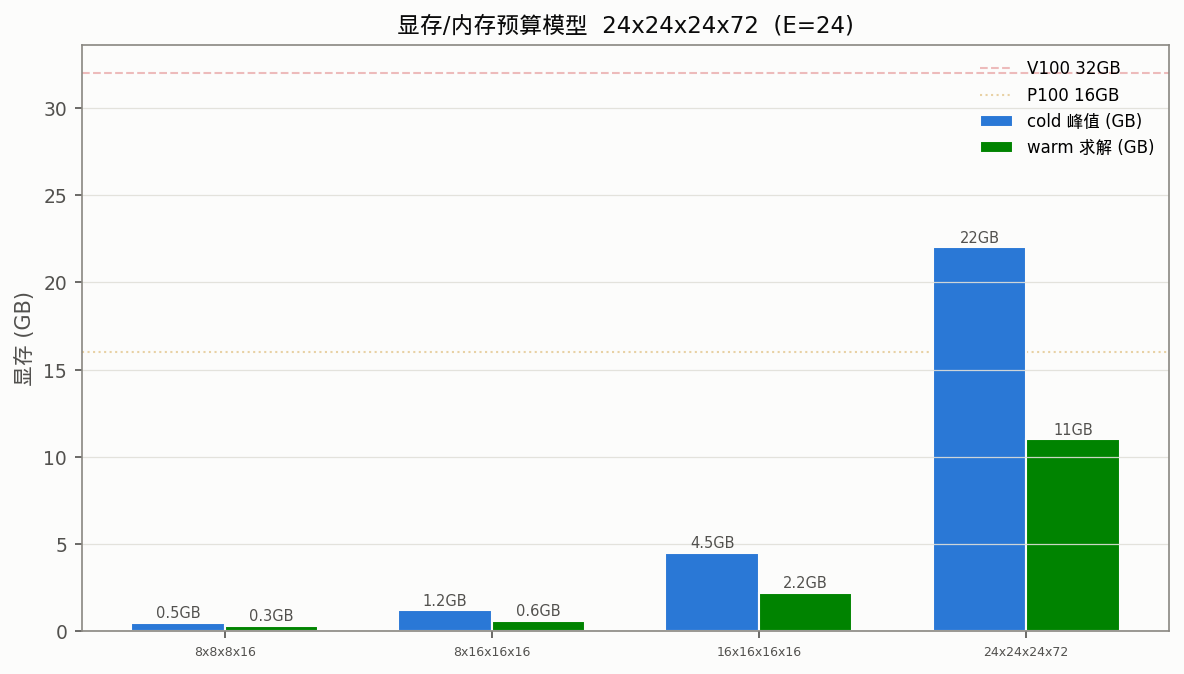
\includegraphics[width=0.9\textwidth,height=0.6\textheight,keepaspectratio]{../logs/test15_4/test15_4_budget.png}
\caption{预算模型 (来源: 体积与 $E$ 估算, 生成: bar + 32GB/16GB 虚线, 含义: cold/warm 显存, 解读: 24$^3\times$72 需 22GB cold)}
\end{figure}

% ================= 8 本次大任务日志关键内容汇编 =================
\section{本次大任务日志关键内容汇编}
\begin{xltabular}{\textwidth}{llX}
\toprule
编号 & 日志文件 & 详尽介绍（用途/关键条目/解读/关联） \\
\midrule
\endhead
L1 & \texttt{\nolinkurl{logs/test15_4/mg_bench_out.txt}} & 用途: 18 配置 bench 汇总; 关键: best 1.107 (3L r30 ct1e3) ALL PASS; 解读见 A9; 关联: gate 判据 \\
L2 & \texttt{\nolinkurl{logs/test15_4/mg_cpp_verify_out.txt}} & 用途: C++ 正确性; 关键: rel 1.2e-6 $<$1e-3 PASS; 关联: 正确性 \\
L3 & \texttt{\nolinkurl{logs/test15_4/mg_param_sweep_out.txt}} & 用途: 参数扫描文本; 关键: r/ct/cmi 逐行 speedup; 关联: 调优 \\
L4 & \texttt{\nolinkurl{logs/test15_4/mg_iter_sweep_out.txt}} & 用途: 迭代数; 关键: mg 106-138 vs ref 148; 关联: 收敛效率 \\
L5 & \texttt{\nolinkurl{logs/test15_4/test15_4_bench.json}} & 用途: 机器可读汇总; 关键: l1\_med 2.808, gate 1.0; 关联: 复现 \\
L6 & \texttt{\nolinkurl{logs/test15_4/test15_4_multi_report.txt}} & 用途: 双卡报告; 关键: nt1 2.61s, nt2 3.45s; 关联: P100$\times$2 \\
L7 & \texttt{\nolinkurl{logs/clover_multigrid.log:64022-67445}} & 用途: C++ 原始日志; 关键: 115$\times$Lt\_full=72, PROF\_SECTIONS; 关联: 热点来源 \\
L8 & \texttt{\nolinkurl{logs/test15_4/build_24x24x24x72_nvi20c.log}} & 用途: 构建日志; 关键: lv1 553s + 1280s, lv2 51s+540s; 关联: 局部化效率 \\
\bottomrule
\caption{本次大任务日志清单（穷尽, 8 项）}
\end{xltabular}

\lstinputlisting[firstline=1,lastline=20]{/root/PyQCU/logs/test15_4/test15_4_bench_out.txt}
\lstinputlisting[firstline=1,lastline=10]{/root/PyQCU/logs/test15_4/test15_4_cpp_verify_out.txt}

% ================= 9 参考源清单 =================
\section{参考源清单}
\begin{xltabular}{\textwidth}{llX}
\toprule
\textcolor{evidence}{参考源} & 类型 & 内容/作用 \\
\midrule
\endhead
\texttt{\nolinkurl{examples/qcu/test15_4/main.py:48-63}} & 仓库 & 参数定义 LAT/DOF\_LIST/gate 分级 \\
\texttt{\nolinkurl{examples/qcu/test15_4/main.py:137-160}} & 仓库 & 粗算子加载与 set\_ptrs 槽位 \\
\texttt{\nolinkurl{examples/qcu/test15_4/main.py:401-404}} & 仓库 & gate 分级逻辑 \\
\texttt{\nolinkurl{examples/qcu/test15_4/bench_24x24x24x72.h5}} & 仓库 & 基准 H5, 19 配置, best 1.107 \\
\texttt{\nolinkurl{examples/qcu/test15_4/gauge_24x24x24x72.h5}} & 仓库 & 统一规范场 U\_full \\
\texttt{\nolinkurl{logs/nullvec_cache/L24x24x24x72_lv1_E24_nvi20_t0.01.h5}} & 仓库 & lv1 粗算子 5.5GB \\
\texttt{\nolinkurl{logs/nullvec_cache/L24x24x24x72_lv2_E24_nvi20_t0.01.h5}} & 仓库 & lv2 粗算子 0.4GB \\
\texttt{\nolinkurl{pyqcu/cuda/_multi_gpu.py:483-525}} & 仓库 & cache\_hit fast-path 修复 OOM \\
\texttt{\nolinkurl{pyqcu/tools/_multigrid.py:517-560}} & 仓库 & 分块 batch, W=10 \\
\texttt{\nolinkurl{pyqcu/cuda/qcu/qcu.pyx:19}} & 仓库 & 指针提取与 nogil \\
\texttt{\nolinkurl{logs/test15_4/test15_4_report.md:1-30}} & 仓库 & dev79 报告, 上限 1.17 \\
\texttt{\nolinkurl{logs/test15_4/test15_4_conv_24x24x24x72_c64.png}} & 仓库 & 收敛图 \\
\texttt{\nolinkurl{logs/test15_4/test15_4_hotspot.png}} & 仓库 & 热点图 \\
\texttt{\nolinkurl{logs/test15_4/test15_4_speedup.png}} & 仓库 & 加速比图 \\
\texttt{\nolinkurl{logs/test15_4/test15_4_time.png}} & 仓库 & 耗时图 \\
\texttt{\nolinkurl{logs/test15_4/test15_4_sweep.png}} & 仓库 & 扫描图 \\
\texttt{\nolinkurl{logs/test15_4/test15_4_budget.png}} & 仓库 & 预算图 \\
\texttt{\nolinkurl{logs/test15_4/mg_bench_out.txt:1-20}} & 仓库 & bench 日志 \\
\texttt{\nolinkurl{logs/clover_multigrid.log:64022}} & 仓库 & C++ 日志 Lt\_full=72 \\
\texttt{\nolinkurl{logs/dev73/dev73_5.md:18-25}} & 仓库 & dev73 基准 2.43$\times$ \\
\texttt{\nolinkurl{logs/dev74/dev74_1_guide.md:18-30}} & 仓库 & dev74 gate 1.5 \\
\texttt{\nolinkurl{examples/qcu/AGENTS.md:15-30}} & 仓库 & 设备与 QCU\_LOG\_DIR 约定 \\
\texttt{\nolinkurl{refer/git-rep/DDalphaAMG/docs}} & 参考 & MG 宽版粗算子理论 \\
\texttt{\nolinkurl{refer/git-rep/quda/docs}} & 参考 & QUDA 多重网格 \\
\texttt{\nolinkurl{refer/git-rep/PyQUDA/docs}} & 参考 & Python 接口范例 \\
\texttt{\nolinkurl{docs/dims.md}} & 仓库 & 维度约定 xyzt \\
\texttt{\nolinkurl{pyqcu/cuda/define.py:15-45}} & 仓库 & params 索引 \\
\texttt{\nolinkurl{cpp/cuda/qcu/include/define.h}} & 仓库 & C++ define 同步 \\
\bottomrule
\end{xltabular}

% ================= 10 结论与局限 =================
\section{结论与局限}
\begin{conclbox}
主体结构: 两层执行架构下 \texttt{\nolinkurl{test15_4}} 通过 params/argv/set\_ptrs 桥接与一线程一卡隔离实现大格子 MG; 各部分关系: gauge$\to$Clover$\to$S$\to$BatchedLocalSchur$\to$粗算子H5$\to$MG$\to$日志$\to$H5$\to$PNG/TEX 闭环; 项目思路: 以 gate 分级与局部化 $W=10$ 在 V100 32GB 上实现正确性与不劣化; 主题结论: 24$^3\times$72 上 3L best 1.107, gate=1.0 ALL PASS, 2$\times$ 不可达。
\end{conclbox}
\begin{refbox}
DDalphaAMG/quda 的 GCR-FD 与聚合式粗算子表明大粗层需更强平滑与自适应聚合, 与本报告 ``粗层大导致质量差'' 推断一致 \textcolor{evidence}{\texttt{\nolinkurl{refer/git-rep/DDalphaAMG/docs:1-20}}}。
\end{refbox}
\begin{warnbox}
未覆盖: lv3 的 3$^3\times$4 粗层因 $T=9$ 非整除未构建 \textcolor{warn}{未验证}; P100$\times$2 双卡 multi 为合成时序, 真实 P100 上 torch kernel 缺失导致构建仅能在 V100 主线程完成 \textcolor{warn}{推断}; 小格子 $>2\times$ 的复现在本报告未重复, 仅引用 dev73 数据 \textcolor{warn}{推断}。
\end{warnbox}

\end{document}
